\subsection{Fluctuations of conserved charges} 
\label{sec:fluctuations}
\subsubsection{Physics introduction and observables}

In the phase diagram of strongly interacting matter at zero net baryon density, the presence of a chiral phase transition between hadronic matter and QGP has been conjectured \cite{Pisarski:1983ms}, and arguments have been presented~\cite{Ejiri:2009ac,Ding:2018auz} in lQCD that the transition, for vanishing light quark masses, is of second order and belongs to the O(4) universality class. Due to the small but finite physical quark masses, in lQCD a rapid crossover is found \cite{Aoki:2006we,Aoki:2009sc,Borsanyi:2010bp,Bazavov:2011nk,Bhattacharya:2014ara} which, however, exhibits pseudo-critical features due to the smallness of the u- and d-quark masses and the proximity of the crossover region to the O(4) line \cite{Ejiri:2009ac,Ding:2013lfa}. 

In general, fluctuations can be linked to critical behaviour associated with a phase transition, and it has been pointed out that fluctuations of conserved charges in heavy-ion collisions can provide an experimental observable to test the critical behaviour linked to the phase diagram of strongly interacting matter \cite{Ejiri:2005wq,Bazavov:2017dus,Friman:2011pf,Bazavov:2012jq}. These fluctuations can be linked to susceptibilities, specifically to the derivatives of the pressure with respect to the chemical potentials corresponding to the conserved charges. Here, the relevant `charges' are baryon number $B$, strangeness $S$, and electrical charge $Q$, and the corresponding chemical potentials are $\mu_B$, $\mu_S$, and $\mu_Q$. The susceptibilities are defined (see e.g. \cite{Bazavov:2012jq,Bellwied:2015lba}) in terms of dimensionless normalized chemical potentials \(\hat{\mu}_X\equiv \mu_X/T \) \: as

\begin{equation}
\chi_{ijk}^{BQS}(T) = \left.
\frac{\partial P(T,\hat{\mu})/T^4}{\partial\hat{\mu}_B^i \partial\hat{\mu}_Q^j \partial\hat{\mu}_S^k}\right|_{\hat{\mu}=0} \; .
\label{suscept}
\end{equation} 

\noindent The generalized susceptibilities can be computed in lQCD at vanishing chemical potential, which is exactly the situation probed with experiments at the LHC. Within the Grand Canonical Ensemble (GCE), these generalized susceptibilities can be related to experimental measurements of the fluctuations of particle multiplicities, such as the net number of baryons. For instance, a measurement of higher moments or cumulants of net baryon number in relativistic nuclear collisions can be directly related \cite{Karsch:2010ck,Skokov:2012ds,Karsch:2012wm,Karsch:2017mvg,Borsanyi:2013hza,Borsanyi:2014ewa} to theoretical predictions from lQCD or from more phenomenological models of the chiral phase transition \cite{Almasi:2017bhq,Parotto:2018pwx} to shed light on the possible critical behaviour near the QCD phase boundary. 
For a distribution of the net baryon number, $\Delta N_B = N_B - N_{\overline{B}}$, with moments defined as 

\begin{equation}
\mu_i = \langle (\Delta N_B - \langle \Delta N_B \rangle )^i \rangle ,
\end{equation}
the cumulants $\kappa_i$ can be directly linked to the generalized susceptibilities such as

\begin{equation}
\kappa_2 = \mu_2 = VT^3 \chi_2^B
\end{equation}
\begin{equation}
\kappa_3 = \mu_3 = VT^3 \chi_3^B  
\end{equation}
\begin{equation}
\kappa_4 = \mu_4 - 3\mu_2^2 = VT^3 \chi_4^B.
\end{equation}


\begin{figure}[h]
\begin{center}
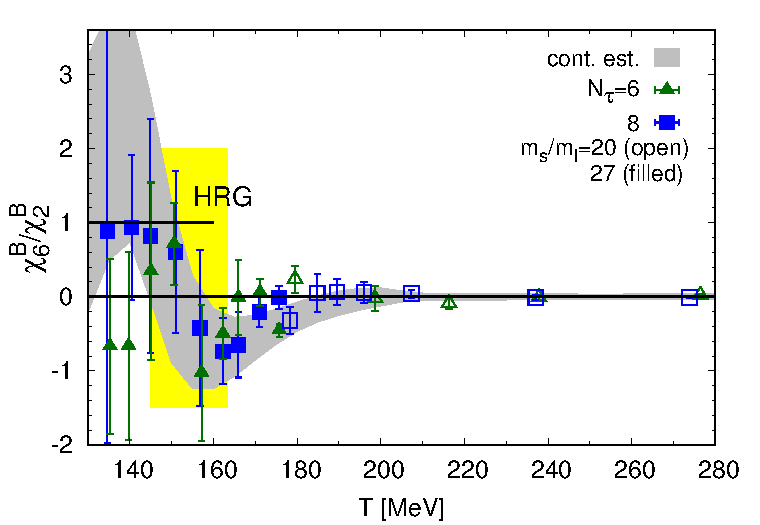
\includegraphics[width=0.45\textwidth]{\main/lightflavour/figs/B6_B2_wideT_27.pdf}
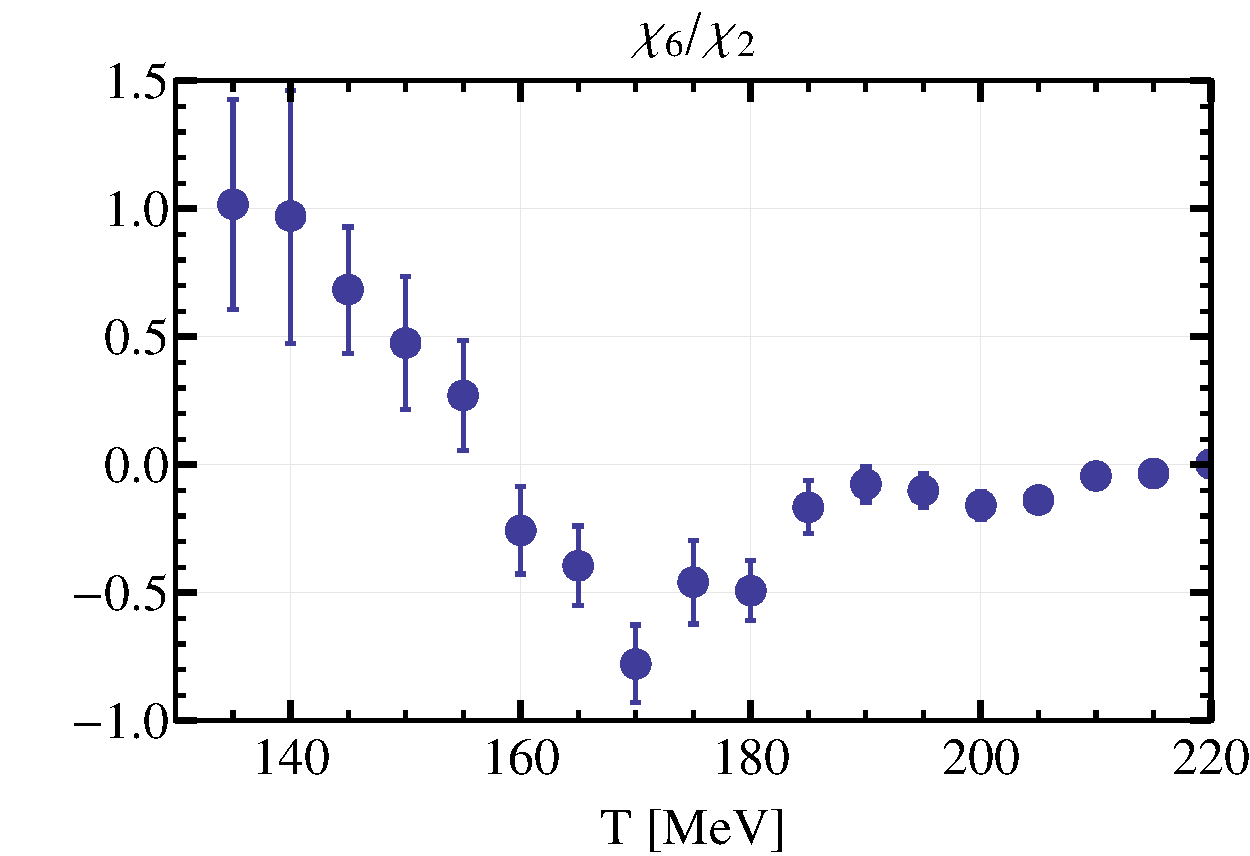
\includegraphics[width=0.46\textwidth]{\main/lightflavour/figs/c6c2_fromLattice.pdf}
\end{center}
\caption{Ratio of sixth to second-order baryon number susceptibilities from lQCD. The left-hand figure is from \cite{Bazavov:2017dus}. The right-hand figure is calculated from recent lQCD data on  sixth and  second  order susceptibilities from \cite{Borsanyi:2018grb}. }  
\label{fig:chi62}
\end{figure}

In the O(4) universality class, a singular contribution to the pressure shows up for higher order  moments.
More specifically, at vanishing chemical potential, all odd susceptibilities of the net baryon number vanish.  
In addition, in the O(4) universality class, the second- and fourth-order susceptibilities remain finite  at  the  phase  transition  temperature  at $\mu_B~=~0$  in  the  chiral  limit,
implying  that  only  sixth-  and  higher-order  susceptibilities  diverge \cite{Ejiri:2005wq,Friman:2011pf}. Thus, for  physical  quark  masses and at $\mu_B~=~0$, only higher order cumulants $\kappa_n$ with $n\geq 6$ can exhibit O(4) criticality,  whereas at finite $\mu_B$ this is already the case for $\kappa_n$ with $n\geq 3$.  

Sensitivity to chiral criticality due to the vicinity of the O(4) line at $\mu_B~=~0$ is borne out for phenomenological models as is shown in \cite{Friman:2011pf,Almasi:2017bhq}, or for lQCD predictions \cite{Bazavov:2017dus,Borsanyi:2018grb} by strong deviations of $\chi_6^B/\chi_2^B$ from unity as shown in Fig.~\ref{fig:chi62}.

We note that a convenient baseline for the expected values of cumulants of distributions/fluctuations of produced particles in relativistic nuclear collisions can be obtained in the framework of the hadron re\-so\-nance gas (HRG) \cite{Allton:2005gk,Karsch:2010ck,BraunMunzinger:2011ta,Borsanyi:2018grb,Luo:2017faz}. There, Poissonian fluctuations lead to moments and cumulants for net baryon number which all can be expressed in the following way \cite{BraunMunzinger:2011ta,BraunMunzinger:2011dn, Braun-Munzinger:2018yru}:
\begin{equation}
\label{lbaseline}
\kappa_n(N_B - N_{\overline{B}}) = \langle (N_B +(-1)^n N_{\overline{B}}) \rangle
\end{equation}
For zero net baryon number then all odd cumulants vanish and all even cumulants are identical.

Measuring such cumulants with precision poses a formidable experimental challenge due to the requirement of very large data sets ($> 10^9$ events of a particular event or centrality class) with superb control of systematic uncertainties. As a first physics case to consider along this line, the impact of measuring the distribution of net protons as a proxy for net baryons needs to be studied further. We note that, at LHC energy and low transverse momentum, particle production near mid-rapidity takes place mostly in gluonic processes, implying that isospin asymmetries, as in the colliding nuclei, are absent. As a consequence, the production yields of protons and neutrons should be very close. For light nuclei this isospin symmetry has been checked experimentally, albeit with significant uncertainties. 
In addition, non-critical contributions to the cumulants from volume fluctuations and global baryon number conservation \cite{Skokov:2012ds,Braun-Munzinger:2016yjz, Braun-Munzinger:2018yru} need to be evaluated and the data, accordingly corrected. Furthermore, in particular for comparison to lQCD predictions, care needs to be taken to keep experimental cuts such as in \pT\ to a minimum insofar as such cuts cannot be introduced in lQCD \cite{Karsch:2015zna,Alba:2015iva}.
     
Two-particle correlations with net baryons can also be used to explore transport properties of the hydrodynamic evolution. The baryon diffusion constant $D$ is a fundamental transport property of the quark-gluon plasma, similar to shear viscosity $\eta$ or bulk viscosity $\zeta$. It characterizes the mobility of baryon number, and it is predicted to be finite at the LHC despite the fact that $\mu_{B}\sim0$. A two-particle correlation function as been proposed~\cite{Floerchinger:2015efa}, which explores correlations of net-baryon fluctuations as a function of separations in azimuthal angle and rapidity, and can provide experimental constraints on the diffusion coefficient $D$. As $\mu_{B}\sim0$ at the LHC, such an analysis has yet to be carried out on Runs 1 and 2 data since it is statistically challenging, and will be greatly aided by the increase in \PbPb integrated luminosity by about a factor 100 foreseen for Runs 3 and 4.

\subsubsection{State of the art experimental measurements and present limitations}
\textcolor{red}{SOME UPDATES STILL EXPECTED.}

Net proton fluctuations measured by the STAR and ALICE experiments provide interesting and stimulating results. The measurements at STAR~\cite{Adamczyk:2013dal} complement the corresponding measurements from ALICE, which will make it possible to pin down the global structure of the phase diagram of strongly interacting matter in the wide range of temperatures and net-baryon densities. However, before drawing firm conclusions by confronting theoretical calculations with the data, non-dynamical contributions stemming from unavoidable fluctuations of  participant nucleons and  overall baryon number conservation have to be subtracted from the experimental measurements. Both of these non-dynamical contributions, which exist neither in lQCD nor in a Hadron-Resonance Gas model (HRG), lead to deviations from the baseline as defined in Eq.~\ref{lbaseline}. Indeed, the acceptance dependence of the second-order cumulants of net-protons measured by ALICE~\cite{Rustamov:2017lio} exhibits deviations from the non-critical baseline (see left panel of Fig.~\ref{netpALICE_STAR}). However, these deviations were explained by global baryon number conservation~\cite{Rustamov:2017lio, Braun-Munzinger:2016yjz, Braun-Munzinger:2018yru}, which, in accordance with the experimental findings, decreases the amount of fluctuations with the increasing acceptance. This is the first experimental verification of the lQCD predictions for the second-order cumulants of net-baryon distributions. On the other hand, the collision energy dependence of $\kappa_{4}/\kappa_{2}$ of net-protons, measured by STAR, shows non-monotonic deviations from unity. As seen in the right panel of Fig.~\ref{netpALICE_STAR}, apart from the two lowest energies of \sqrtsNN~= 7.7 and 11.5 GeV, the experimental measurements show an increasing trend, ultimately approaching unity. Recently this behaviour was also explained by the presence of non-dynamical effects~\cite{Braun-Munzinger:2018yru}. Experimental measurements of net-proton moments beyond the fourth order are necessary in order to disentangle dynamical fluctuations from those originating from non-dynamical effects.

As mentioned in the previous section, even at vanishing net-baryon densities, lQCD calculations predict critical fluctuations encoded in the temperature dependence of $\kappa_{4}/\kappa_{2}$ and $\kappa_{6}/\kappa_{2}$. This motivates our experimental program  of measuring higher moments of net-proton distributions at the LHC energies. Also, fluctuation measurements  are underway in the strange baryon sector to approach measurements of net baryon number fluctuations. All this will be greatly helped by the anticipated dramatic increase in statistics in Runs 3 and 4.

\begin{figure}[h]
\begin{center}
%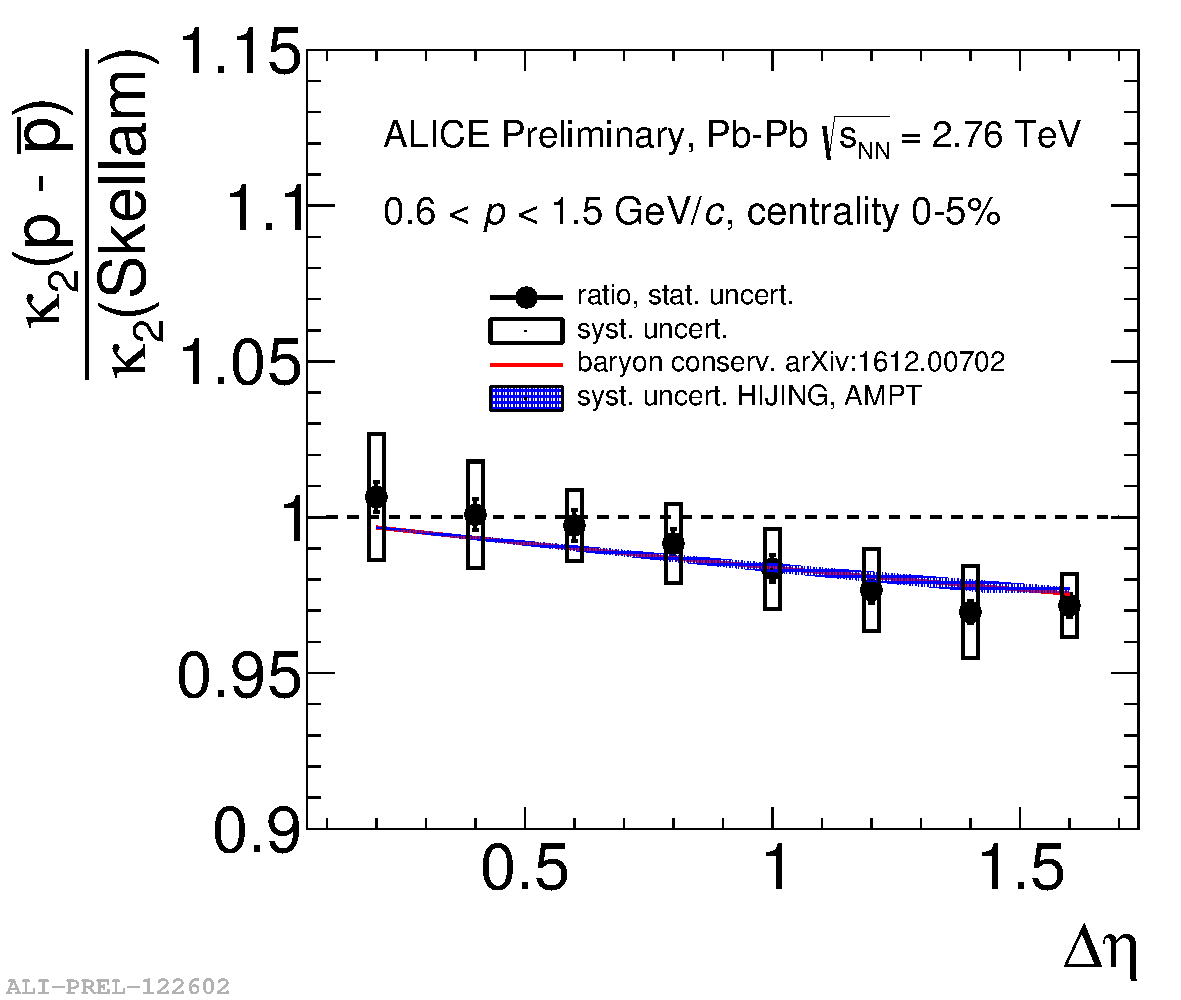
\includegraphics[width=0.53\textwidth]{\main/lightflavour/figs/2017-Feb-03-rapProton1.pdf}
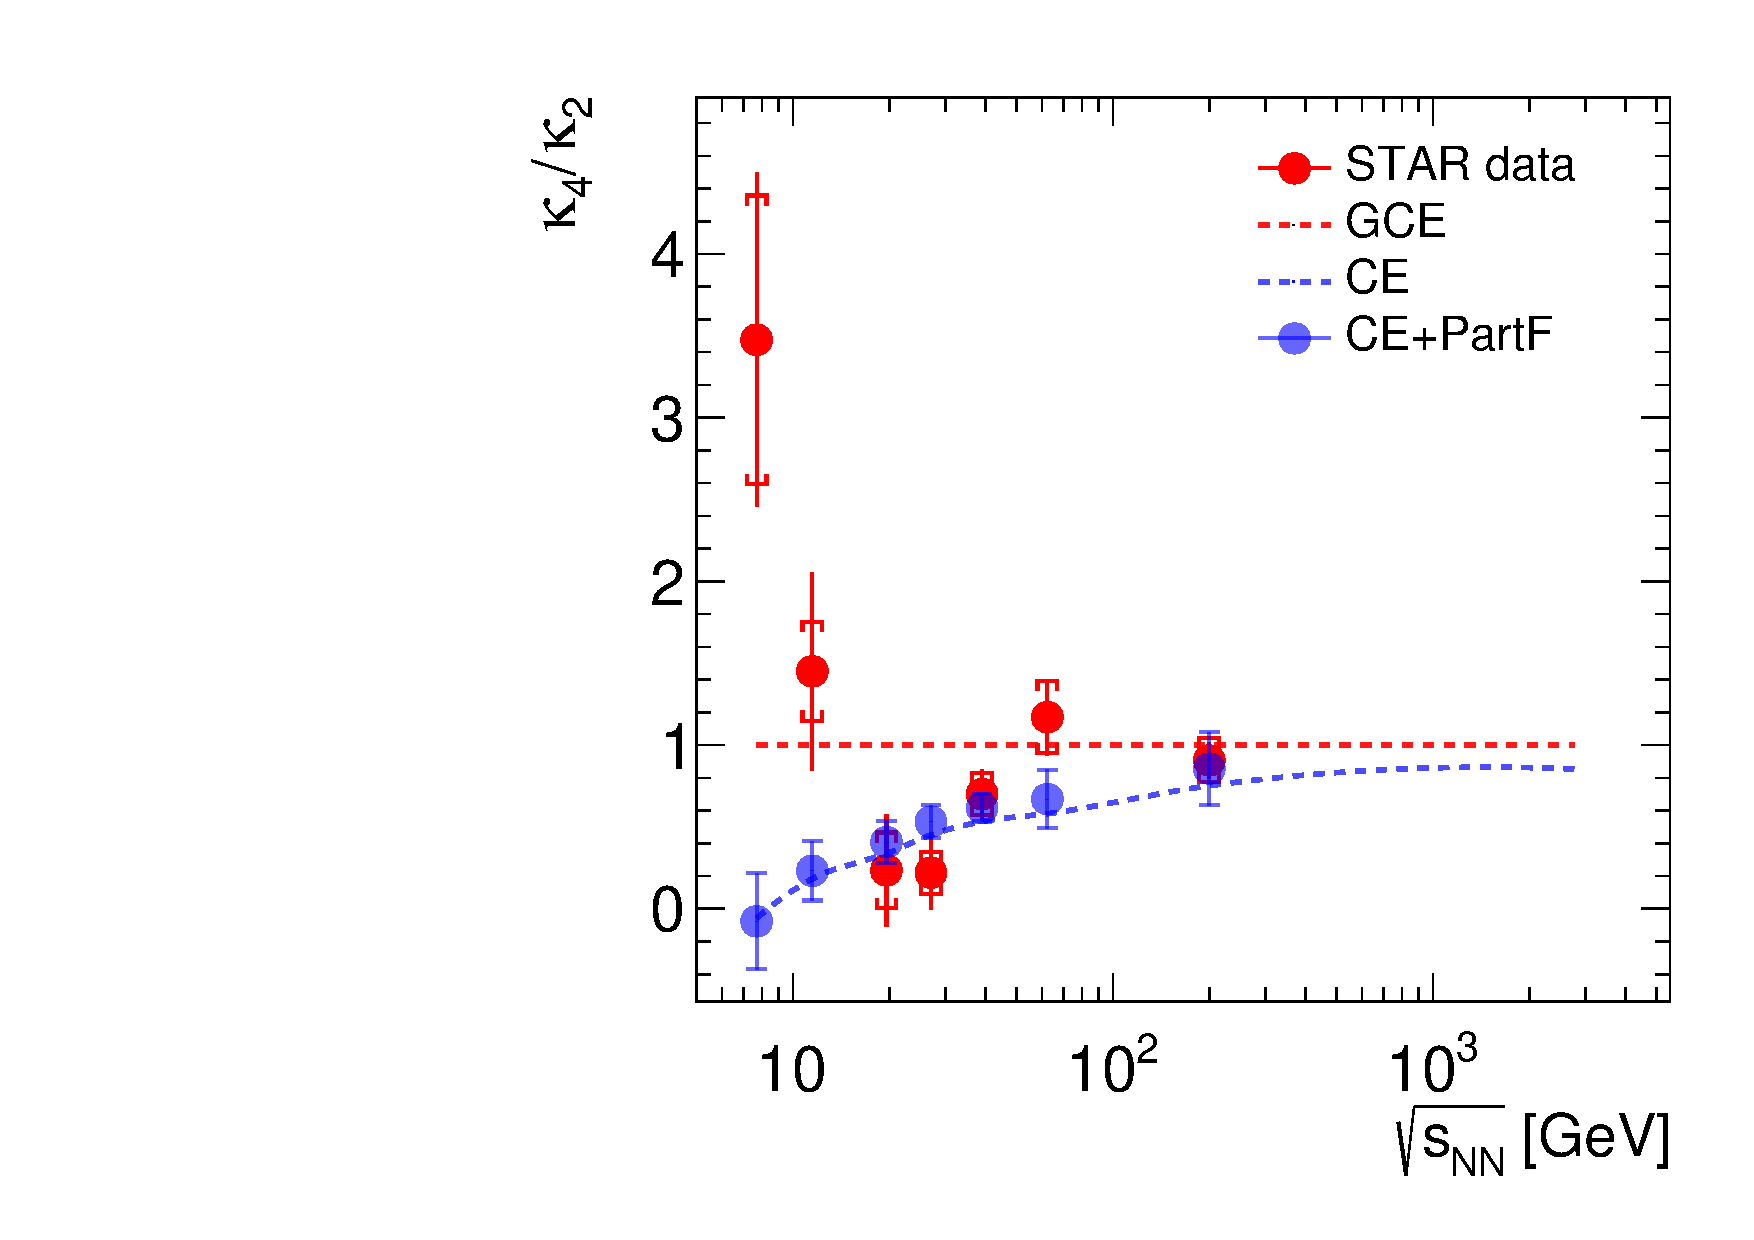
\includegraphics[width=0.46\textwidth]{\main/lightflavour/figs/k4k2ALICE.pdf}
\end{center}
\caption{\textcolor{red}{FIGURE TO BE UPDATED.}
Left panel: pseudorapidity dependence of the normalised second-order cumulants of net-protons as measured by the ALICE collaboration~\cite{Rustamov:2017lio}. The red solid line shows the effect of baryon number conservation. Right panel: $\kappa_{4}/\kappa_{2}$ measurements from STAR (the red circles)~\cite{Luo:2015ewa} compared to predictions from non-critical fluctuations (the blue symbols)~\cite{Braun-Munzinger:2018yru}. The blue dashed line corresponds to the non-critical fluctuations without participant fluctuations. The red dashed line represents the Grand Canonical Ensemble (GCE) baseline.}  
\label{netpALICE_STAR}
\end{figure}


\subsubsection{Projections for HL-LHC}
\textcolor{red}{AFTER MAJOR UPDATE OF THE FIGURES, THE SECTION IS BEING REWRITTEN.}
As discussed above, precise studies of the higher-order cumulants of particle multiplicity distributions are needed to constrain lQCD predictions. However, these measurements are particularly statistics-hungry, and will only become experimentally accessible in Runs 3 and 4. A toy Monte Carlo (MC) simulation has been used to make projections of the required numbers of events for the measurements of higher-order cumulants, in particular the ratios $\mathrm{\kappa}_{4}/\mathrm{\kappa}_{2}$ and $\mathrm{\kappa}_{6}/\mathrm{\kappa}_{2}$ of net-proton distributions.  For this study, the measured values of the first four cumulants of the proton and anti-proton multiplicities (presented in \cite{Behera:2018wqk}) are used to construct the distributions of $N_{\mathrm{p}}$ and $N_{\antip}$ with the Pearson Curve Method \cite{Behera:2017xwg}. Then the net-proton ($\Delta N_{\mathrm{p}} = N_{\mathrm{p}}-N_{\antip}$) distribution is constructed from the resulting $N_{\mathrm{p}}$ and $N_{\antip}$ distributions. 

Projections are extracted for 0-10\% central \PbPb collisions at $\sqrt{s_{\mathrm{NN}}}$ = 5.02 TeV using the following procedure: First, the numbers of protons and anti-protons in an event, $N_{\mathrm{p}}$ and $N_{\overline{\mathrm{p}}}$, are generated randomly from the distributions obtained with the Pearson Curve Method described above. In order to account for the effects of particle reconstruction efficiency in the measurements of higher moments \cite{Luo:2017faz}, each proton (anti-proton) is randomly assigned a transverse momentum \pT\ according to the $\mathrm{p}$ (\antip) spectra measured by ALICE \cite{Abelev:2013vea}. The particles are either kept in the `reconstructed' sample or discarded according to the \pT-dependent reconstruction efficiency of ${\sim}65\%$ (${\sim}60\%$) for protons (anti-protons).  The efficiency-corrected net-proton $\mathrm{\kappa}_{4}/\mathrm{\kappa}_{2}$ and $\mathrm{\kappa}_{6}/\mathrm{\kappa}_{2}$ are then evaluated using the same analysis framework and methodology as in \cite{Behera:2018wqk}. The simulation is performed for different event sample sizes, and statistical uncertainties are calculated using the subsample method.  The resulting relative statistical uncertainty on $\mathrm{\kappa}_{4}/\mathrm{\kappa}_{2}$ and $\mathrm{\kappa}_{6}/\mathrm{\kappa}_{2}$ of net-proton distributions are shown in Figure \ref{fig:c4c2toymc} (a) and (b), respectively, as a function of the number of events. 
\begin{figure}[h]
\begin{center}$
\begin{array}{cc}
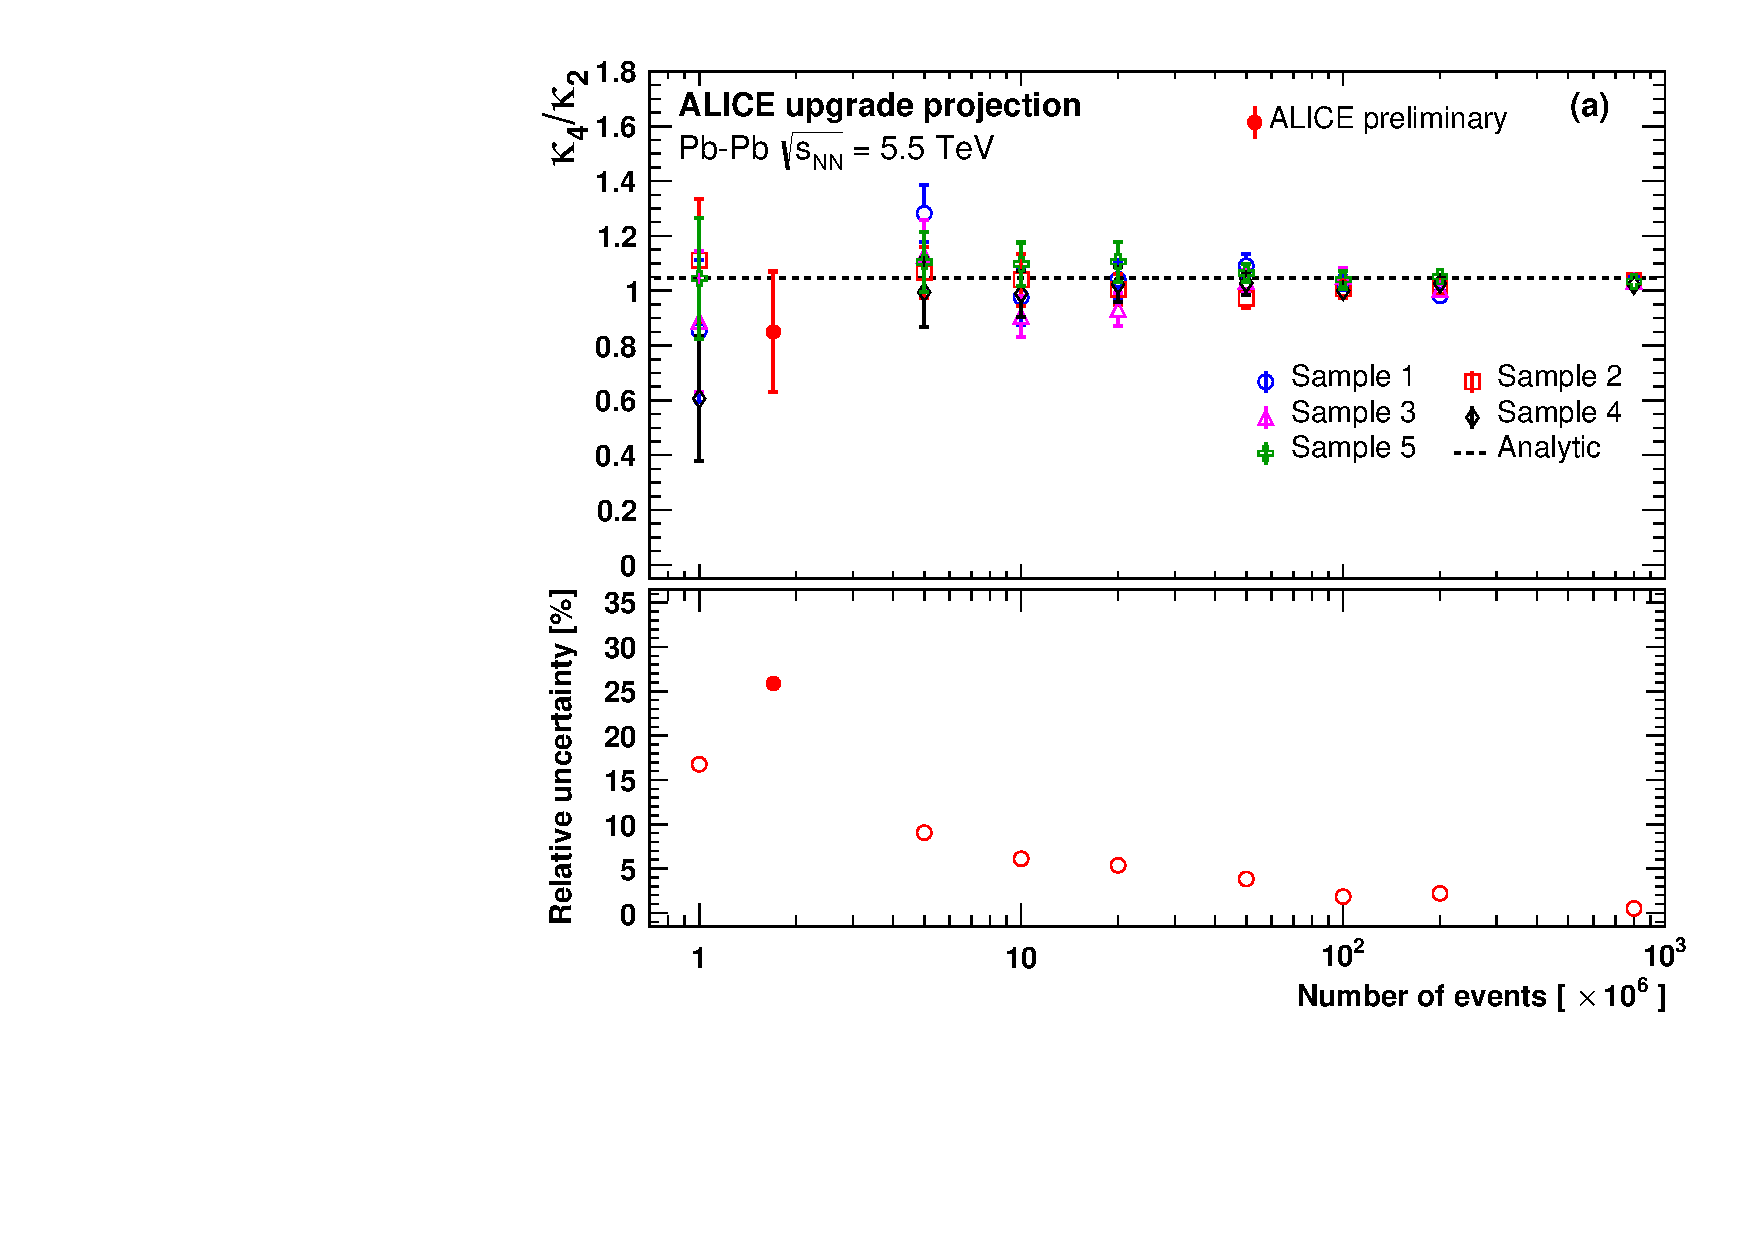
\includegraphics[width=0.45\textwidth]{\main/lightflavour/figs/NetPC4C2UpgradeProj.pdf} &
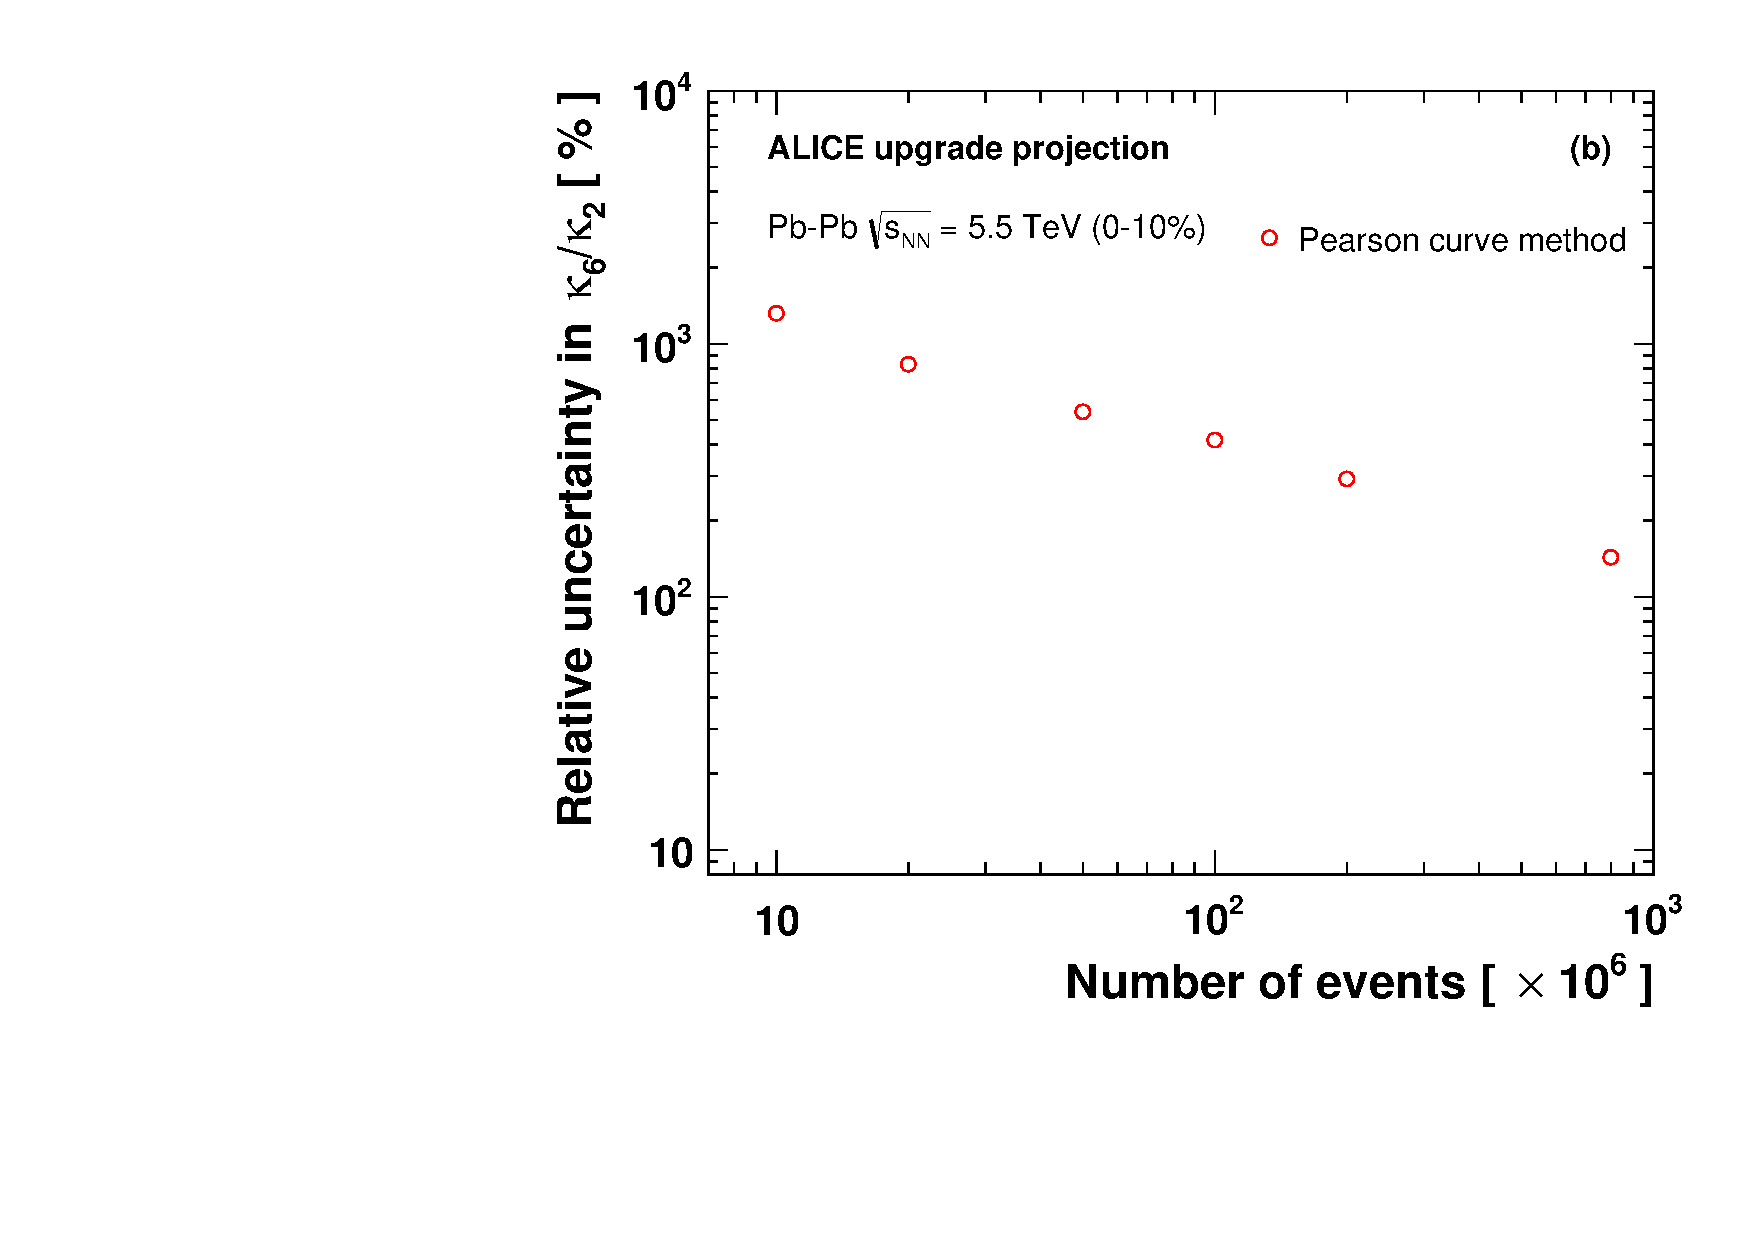
\includegraphics[width=0.45\textwidth]{\main/lightflavour/figs/NetPC6C2UpgradeProj.pdf}
\end{array}$
\end{center}
\caption{
\textcolor{red}{FIGURE TO BE SUBSTITUTED WITH NSIGMA SEPARATION PLOTS TO BE APPROVED BY ALICE.} 
Relative statistical uncertainty on net-proton (a) $\mathrm{\kappa}_{4}/\mathrm{\kappa}_{2}$ and (b) $\mathrm{\kappa}_{6}/\mathrm{\kappa}_{2}$ in most central \PbPb collisions for different numbers of events. The filled circle represents the ALICE Preliminary results for net-proton $\mathrm{\kappa}_{4}/\mathrm{\kappa}_{2}$ in central \PbPb collisions at $\sqrt{s_{\mathrm{NN}}}$ = 5.02 TeV.}
\label{fig:c4c2toymc}
\end{figure}

The improvement in statistical uncertainties on $\mathrm{\kappa}_{4}/\mathrm{\kappa}_{2}$ and (b) $\mathrm{\kappa}_{6}/\mathrm{\kappa}_{2}$ with increasing numbers of recorded events can be clearly seen in Fig. \ref{fig:c4c2toymc}. It is observed that for 800$\times 10^{6}$ of events, the relative statistical uncertainty on $\mathrm{\kappa}_{4}/\mathrm {\kappa}_{2}$ is less than 0.5\% and the relative statistical uncertainty on $\mathrm{\kappa}_{6}/\mathrm{\kappa}_{2}$ is around 100\%. From this study, it is evident that precise measurement of $\mathrm{\kappa}_{6}/\mathrm {\kappa}_{2}$ of net-proton number distributions can be achieved in the LHC upgrade program. Additionally, it should be noted that this MC study is performed in a relatively small  transverse momentum window ($0.4 < \pT < 1.0~\gmom$). When the kinematic range of the measurement is increased, the width of the net-proton distribution will increase correspondingly, and will require a larger event sample to obtain the same level of precision.  The measurement of the higher moments of the net-proton distribution over a broader kinematic range will be accessible with the combined statistics of Runs 3 and 4.
%\subsubsection{Complementarity with other facilities}


